%%
% TUM Corporate Design LaTeX Templates
% Based on the templates from https://www.tum.de/cd
%
% Feel free to join development on
% https://gitlab.lrz.de/tum-templates/templates
% and/or to create an issue in case of trouble.
%
% tum-presentation class for scientific talks, thesis presentations, ...
%
%%

%\documentclass[4to3]{tum-presentation}
%\documentclass[navsym]{tum-presentation}
%\documentclass[nothreeliner]{tum-presentation}
%\documentclass[handout,4on1]{tum-presentation}
%\documentclass[handout,2on1]{tum-presentation}
%\documentclass[handout]{tum-presentation}
\documentclass{tum-presentation}

\addbibresource{literature.bib}

\title[Research Internship]{Research Internship with RCS@TUM}
\subtitle{Implementation of tiny machine learning models on microcontrollers}
\author[Philipp v. K.]{\textbf{Philipp van Kempen}}
\institute[]{Department of Electrical and Computer Engineering,
  Technical University of Munich (TUM)}
\date{\textbf{24.08.2020 - 25.10.2020}}

\footline{\insertshortauthor~|~\insertshorttitle}

\usepackage{multirow}
%\usepackage[table]{xcolor}
\usepackage[utf8]{inputenc}
\usepackage{multirow}
\usepackage{hhline}
\usepackage{colortbl}
\usepackage{multicol}
\usepackage{caption}
\usepackage{subcaption}
\usepackage{hyperref}

\begin{document}

\begin{frame}[noframenumbering]
  \titlepage
\end{frame}

\begin{frame}
  \frametitle{Motivation}

  \begin{figure}[h]
\centering
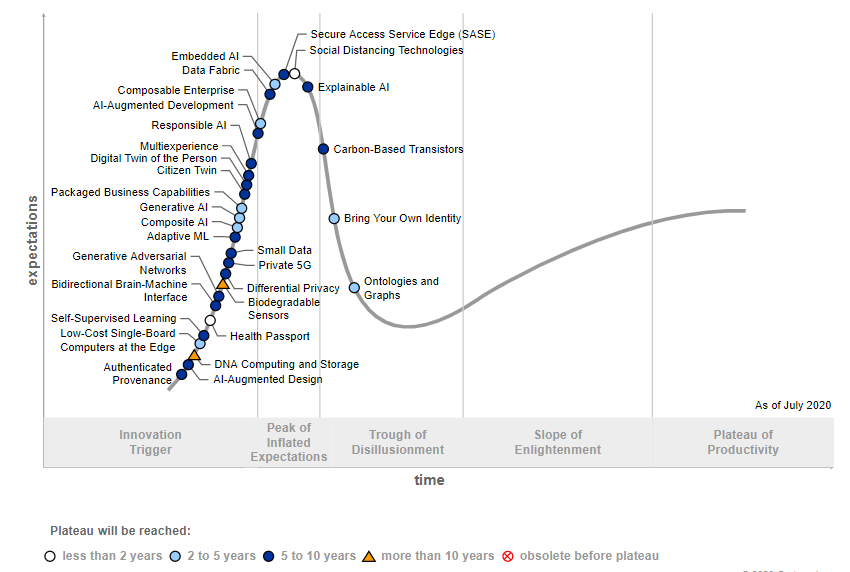
\includegraphics[width=0.45\textwidth]{figures/2020_08_23_medialist_gartner_hype_cycle_2020.png}
\caption{2020 Gartner Hype Cycle\footnote{\url{https://www.gartner.com/smarterwithgartner/5-trends-drive-the-gartner-hype-cycle-for-emerging-technologies-2020/}}}
\label{fig:gartner2020}
\end{figure}

\end{frame}

\begin{frame}

\centering{
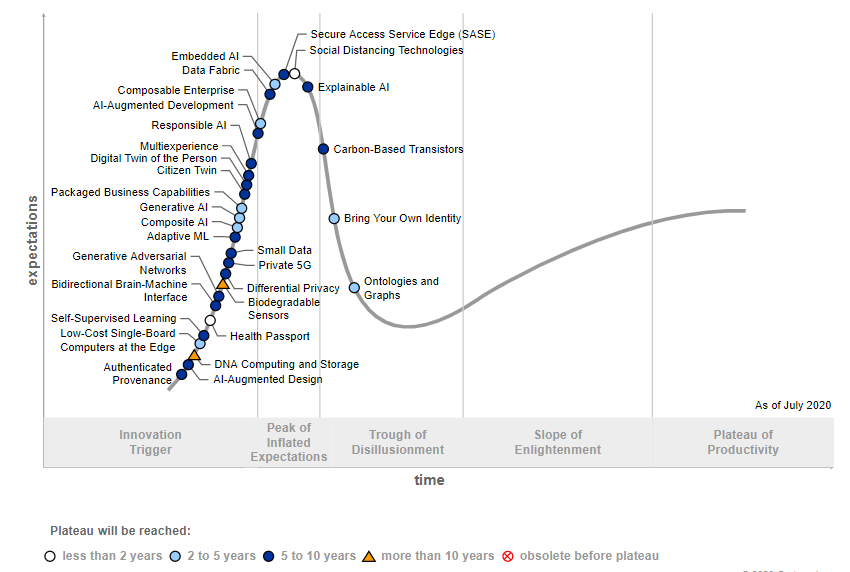
\includegraphics[width=0.7\textwidth]{figures/2020_08_23_medialist_gartner_hype_cycle_2020.png}}

\end{frame}

\begin{frame}
  \frametitle{Goals}
  
  \begin{itemize}
      \item 9 weeks
      \item Support Electronic System Level (ESL) research group (EDA+RCS)
      \item Implement reference implementations of TinyML models on STM32 Hardware
      \item Work based on previous attempts by Alex Hoffman
      \item Extend toolchain with new features and documentation
      \item Summarize results at the end of the internship
  \end{itemize}

\end{frame}

\begin{frame}
  \frametitle{Steps}
\vspace{-5em}
  \begin{figure}[h]
\centering
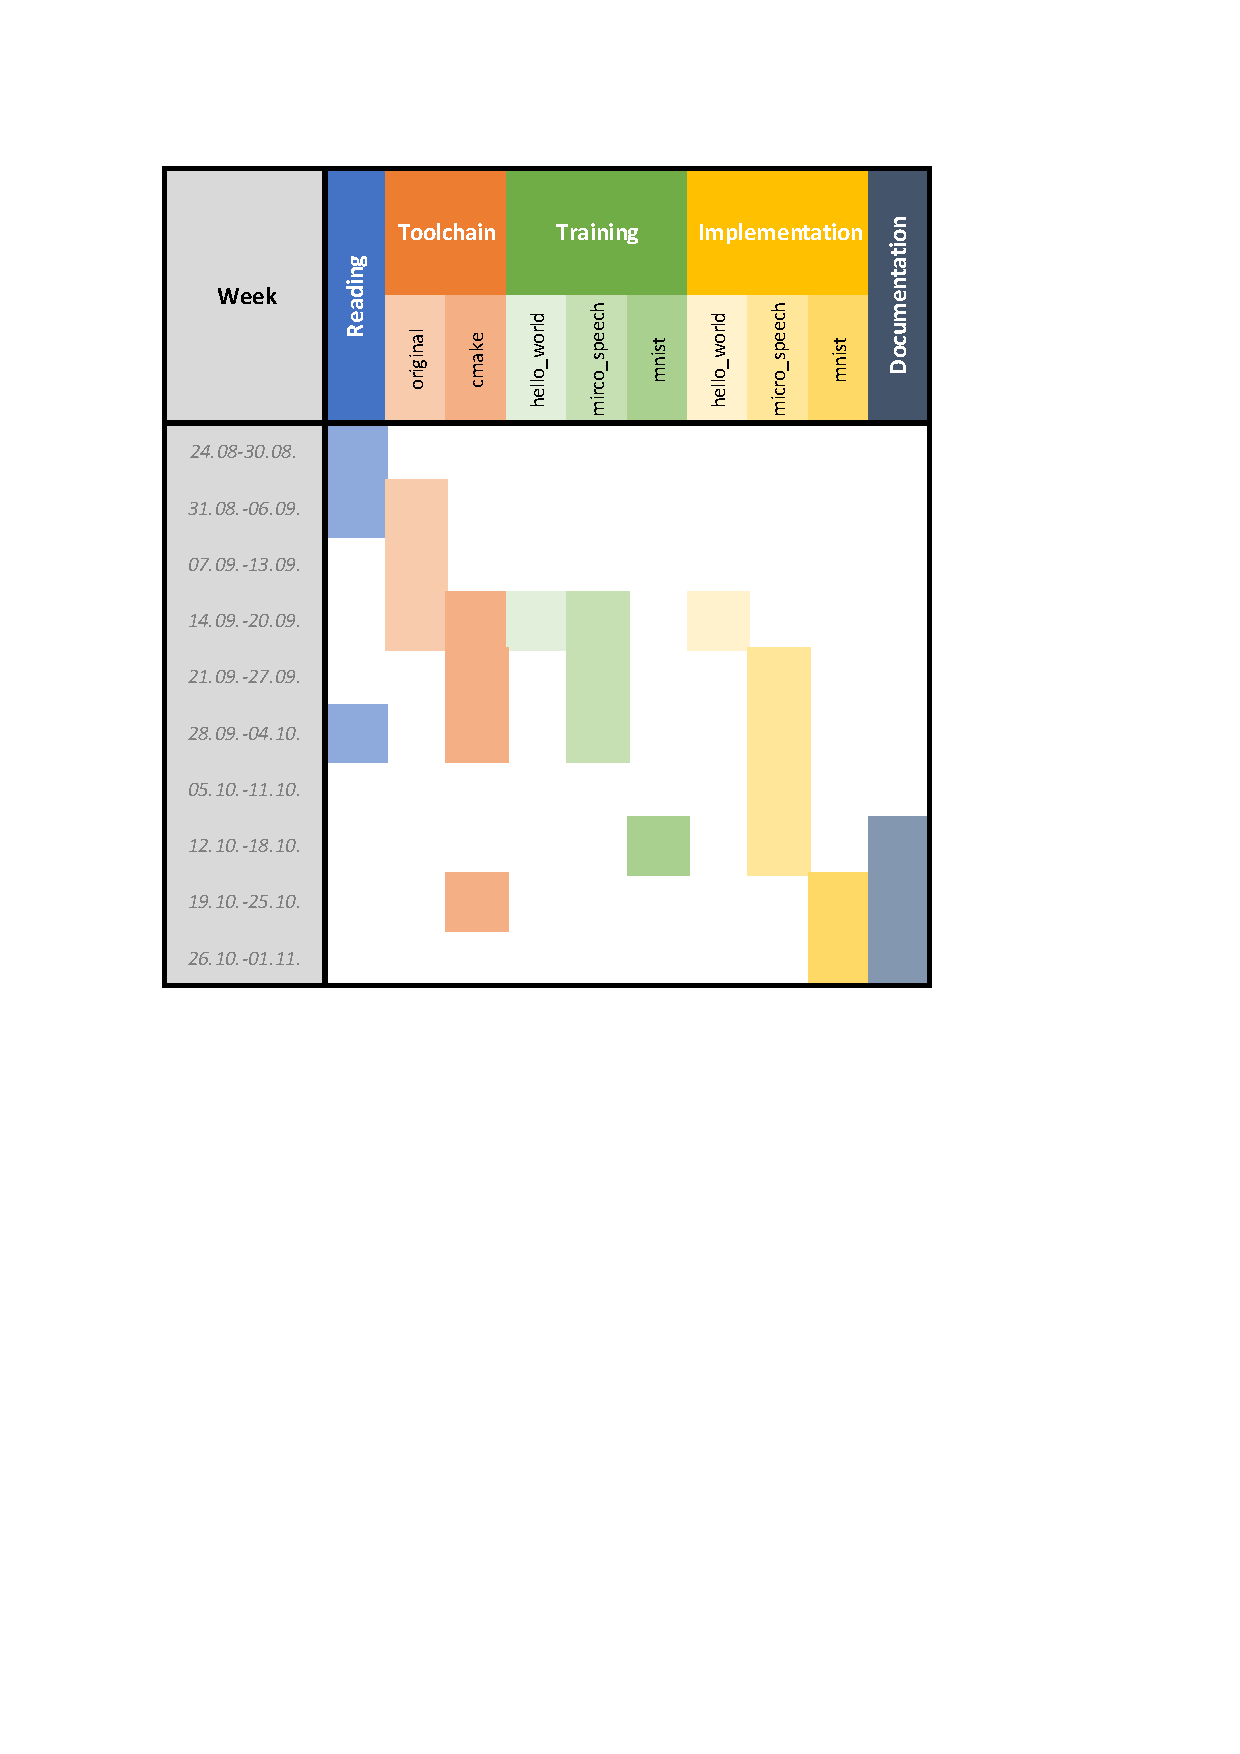
\includegraphics[scale=0.8]{figures/fp_report_plan.pdf}
\caption{Schedule}
\label{fig:schedule}
\end{figure}

\end{frame}

\begin{frame}
  \frametitle{Reading}

  The book by Pete Warden and Daniel Situnayake introduces the usage of the Tensorflow Lite for Microcontrollers (TFLM) framework in a very detailed way. Two of the practical applications, which are all referencing examples located in the Tensorflow source tree, are especially interesting as they are supported a a large number of platforms:

\begin{itemize}
    \item \textbf{Hello World:} A very simple model designed to approximate the value in the trigonometric sine function for a given x-value. As the memory and performance requirements for running this program are very low, it is often used to teach the basics of machine learning.
    \item \textbf{Micro Speech:} Inspired by voice assistants found in devices like smartphones, TVs,... which are able to detect full sentences of human speech via a microphone, this model can classify the voice commands 'yes' and 'no'. Those models, which can only detect single words are often refered as Keyword-Spotting (KWS) models. Running those models on low-power MCUs in embedded devices allows to wake up a larger processor if certain commands are detected as there accuracy alone is often not good enough for reliable results. 
\end{itemize}

In addition to the book, the official documenatation of Tensorflow was a great resource to git started with the topic. It was especially helpful as it contains information for old the latest versions 2.3 of the framework as well as for Tensorflow 1.5 which is still used often in many older models.

\end{frame}

\begin{frame}
  \frametitle{Toolchain}

\begin{itemize}
    \item CMake based
    \item Initially developed by Konstantin Oblaukhov \footnote{TODO}, Improved and extended by Alex Hoffman \footnote{TODO}
    \item Reference Application: \lstinline{STM3240G-EVAL-TensorFlow-MNIST}
    \item Some workarounds required to fix upstream bugs
\end{itemize}

\begin{figure}[h]
     \centering
     \begin{subfigure}[b]{0.49\textwidth}
         \centering
         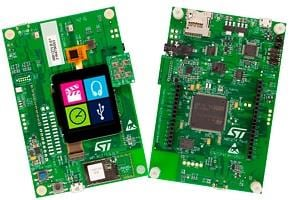
\includegraphics[width=0.45\textwidth]{figures/disco_f413h.jpg}
         \caption{STM32F413H-DISCOVERY}
         \label{fig:stm32f4}
     \end{subfigure}
     \hfill
     \begin{subfigure}[b]{0.49\textwidth}
         \centering
         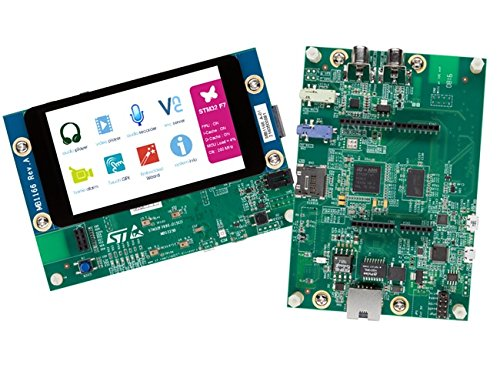
\includegraphics[width=0.45\textwidth]{figures/disco_f769i.jpg}
         \caption{STM32F769I-DISCOVERY}
         \label{fig:stm32f7}
     \end{subfigure}
        \caption{Target Boards}
        \label{fig:boards}
\end{figure}

\end{frame}

\begin{frame}
  \frametitle{Training}
  
  \begin{itemize}
      \item Training scripts: interactive notebooks hosted on Google Colaboratory\footnote{\url{https://colab.research.google.com}}
      \item Deployment on Microcontrollers:
      \begin{itemize}
          \item Quantization
          \item Optimizartions
          \item Conversion to TFLite
          \item Interpreter vs. Compiled offline model
      \end{itemize}
  \end{itemize}
  \vspace{-5em}
  \hspace{20em}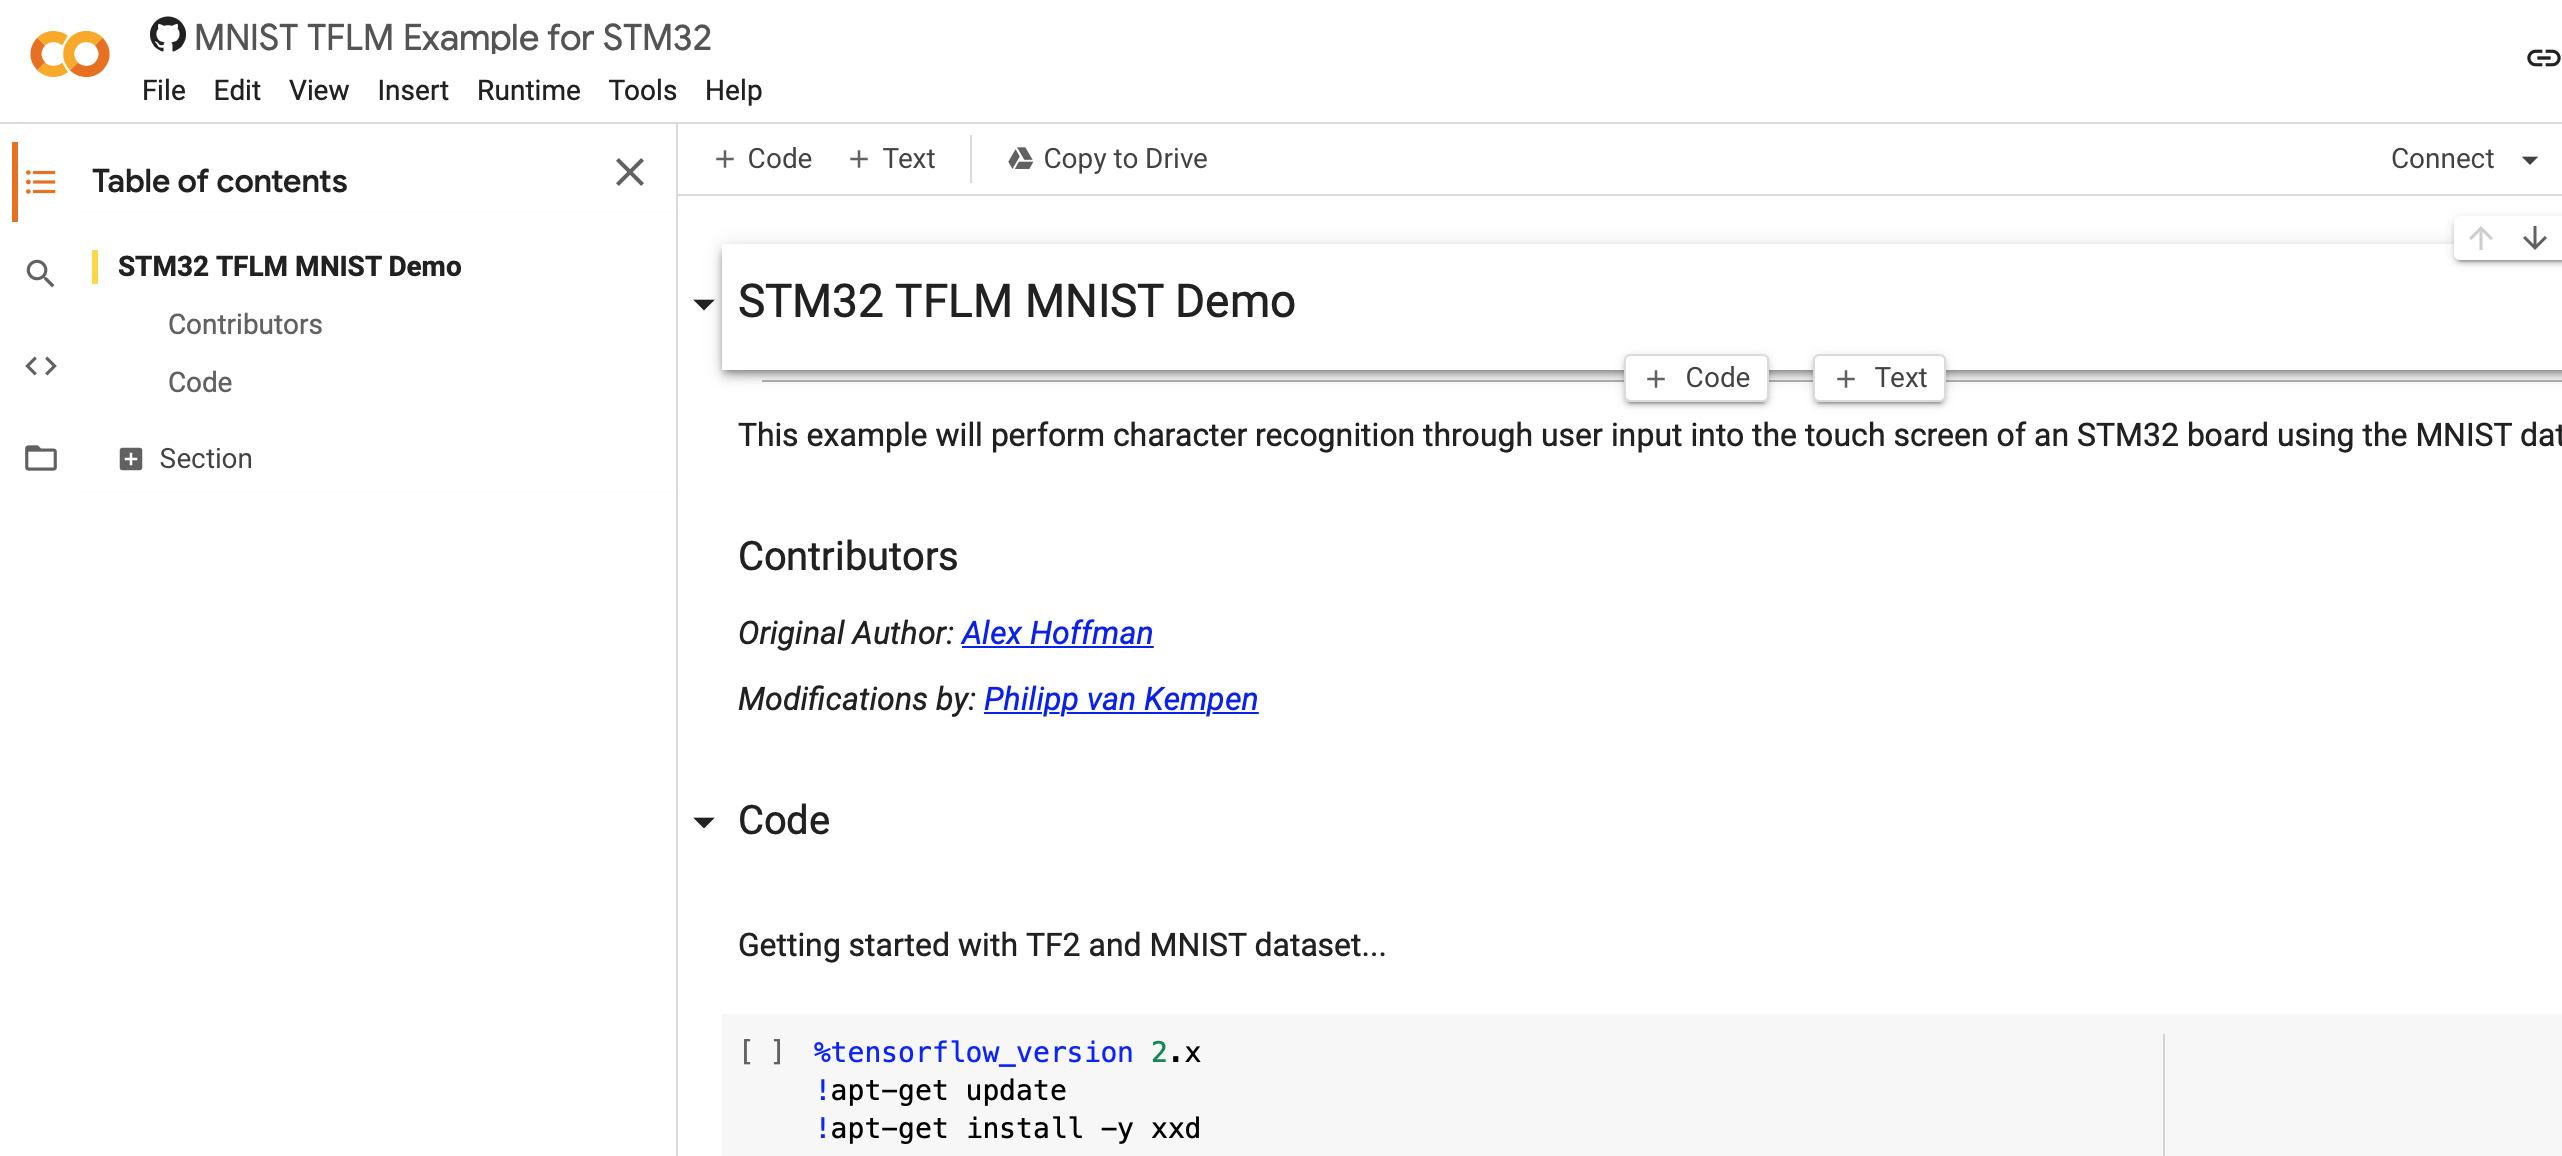
\includegraphics[width=.7\textwidth]{figures/screen_colab.png}
\end{frame}

\begin{frame}

\vspace{-2em}
\begin{figure}[h]
     \centering
     \begin{subfigure}[b]{0.3\textwidth}
         \centering
         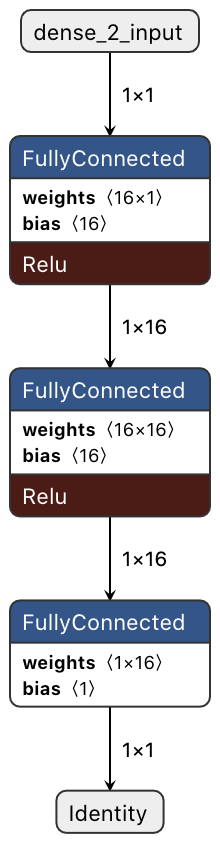
\includegraphics[width=0.3\textwidth]{figures/hello_world_graph.png}
         \caption{Hello World}
         \label{fig:netron_hello_world}
     \end{subfigure}
     \hfill
     \begin{subfigure}[b]{0.3\textwidth}
         \centering
         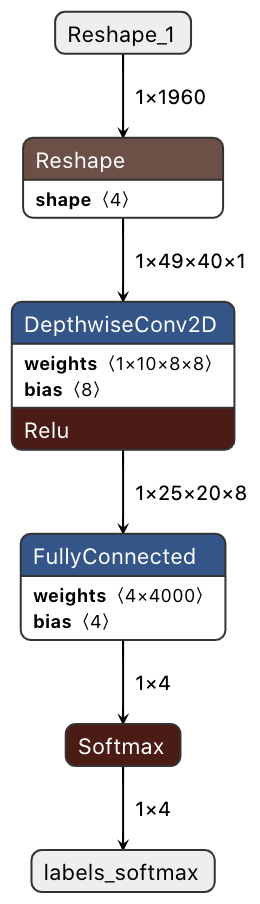
\includegraphics[width=0.4\textwidth]{figures/micro_speech_graph.png}
         \caption{Micro Speech}
         \label{fig:netron_mirco_speech}
     \end{subfigure}
     \hfill
     \begin{subfigure}[b]{0.3\textwidth}
         \centering
         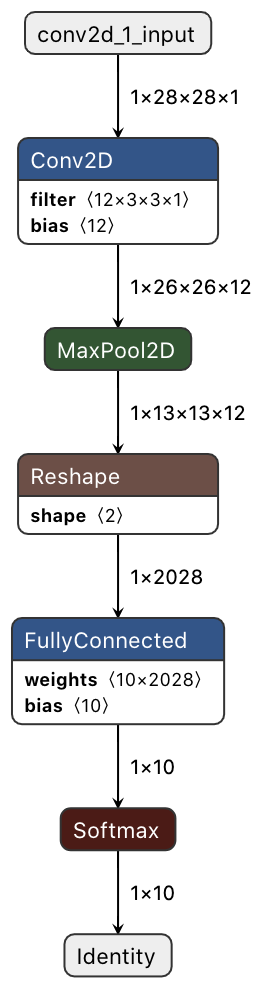
\includegraphics[width=0.4\textwidth]{figures/mnist_graph.png}
         \caption{MNIST}
         \label{fig:netron_mnist}
     \end{subfigure}
        \caption{TFLite Model Graphs per Example}
        \label{fig:netron}
\end{figure}

\end{frame}

\begin{frame}
  \frametitle{Implementation}


Most of the Hello World Demo was running out of the box after the toolchain was updated to be compatible with the latest tensor flow version.

Shortly the first example was running an initial version of a custom benchmarking module was added to the source code which allows to extract execution times of several parts of the main program loop.


The hardest challenge of the Micro Speech example was streaming the input samples for the network in real-time which requires a sufficient execution speed of the four main processes:

\begin{itemize}
    \item \textbf{Feature Generation:} Uses quite large ring-buffers to fit multiple time slots. If the main loop takes to long for one iteration, the buffer size has to be increased to prevent an overflow. Spectrogram-slices are generated with the new samples.
    \item \textbf{Invoke Network:} A set of spectrogram slices is feed into the the network input. The quantized output is an array of signed chars representing a probability of the four classes \lstinline{yes,no,unknown,silence}
    \item \textbf{Post processing Results:} To reduce false positives and handle fluctuations a moving average has to be applied to the history of network outputs. Combined with thresholds and other parameters the detected class of command with the respective probability is returned 
    \item \textbf{Command Responding:} If there is a new command detected, the result is displayed on the screen and/or printed on the serial terminal. 
\end{itemize}

After the microphone functionality was added and the buffer size tuned the model was not responsive at all. It was unclear if the reason for this issue was a to slow processor but at this point the development was shifted to the faster F7 Board. In the meantime, by enabling the support of CMSIS-NN the execution time of the Invoke step was drastically reduced resulting in a higher sample throughput. 

The final step which was required to achieve meaningful results with the application was reducing thresholds and tuning timing constants an the post processing step. In fact, this lead to more wrong detections but at least allowed to detect some correct samples in the end.

To find out if the rather bad performance of the network was cause by the microphone samples being too different compared to the original data set much time was invested adding the ability to provide samples from WAV-files via the on-board SD-card slot. As the manufacturer libraries for the audio codecs did not support playing mono audio. The original 1 second WAV files had to be converted to stereo files beforehand with a custom script.


The well-known MNIST dataset contains ten thousands of hand written digits. They have a quite small resolution and only feature grayscale values to reduce the size and therefore the complexity of the samples.

To use feed digits written via a touchscreen into the network some prepossessing is needed:

\begin{itemize}
    \item Find a suitable brush size (circle radius) for the input
    \item Interpolate between inputs to get a smoother line
    \item Downscale the input image to 28x28 pixels with  a proper filter
    \item Convert the color space of the display to 8 bpp grayscale
    \item Invert the color spectrum (whit on black instead of black on white)
\end{itemize}

Similar to the MNIST implementation SD-Card support for feeding original samples instead of touchscreen data was also added. Scripts to generate board-compatible BMP files are provides with the source code. 

While some of the predictions have been very accurate the network as not capable some digits neither with original samples nor with touchscreen inputs. This leads to the conclusion that the model architecture needs some further tuning.

As the TFLite Micro currently does not support unsigned 8 bit quantization the training script had to be modified to use signed values between -128 and 127. This fact also had to be considered when preparing the input tensor for the network.

Figure \ref{fig:gifs} shows the examples in running on the actual hardware. Animated versions of these graphics can be found in the respective repository!

%\begin{figure}[h]
%     \centering
%     \begin{subfigure}[b]{0.3\textwidth}
%         \centering
%         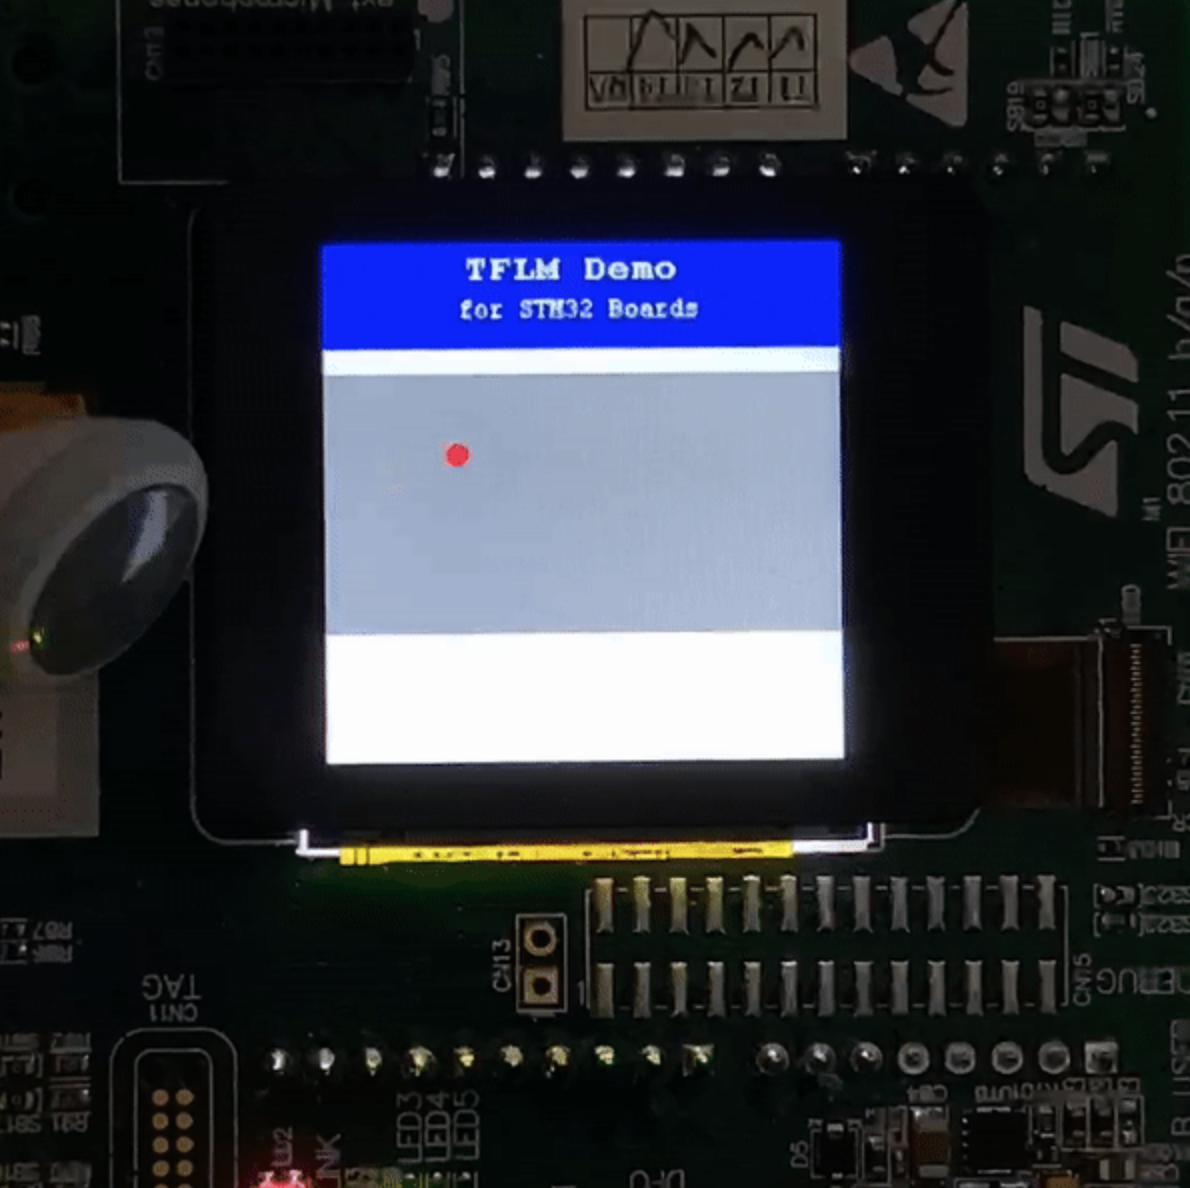
\includegraphics[width=0.8\textwidth]{figures/hello_world_gif.png}
%         \caption{Hello World}
%         \label{fig:gif_hello_world}
%     \end{subfigure}
%     \hfill
%     \begin{subfigure}[b]{0.3\textwidth}
%         \centering
%         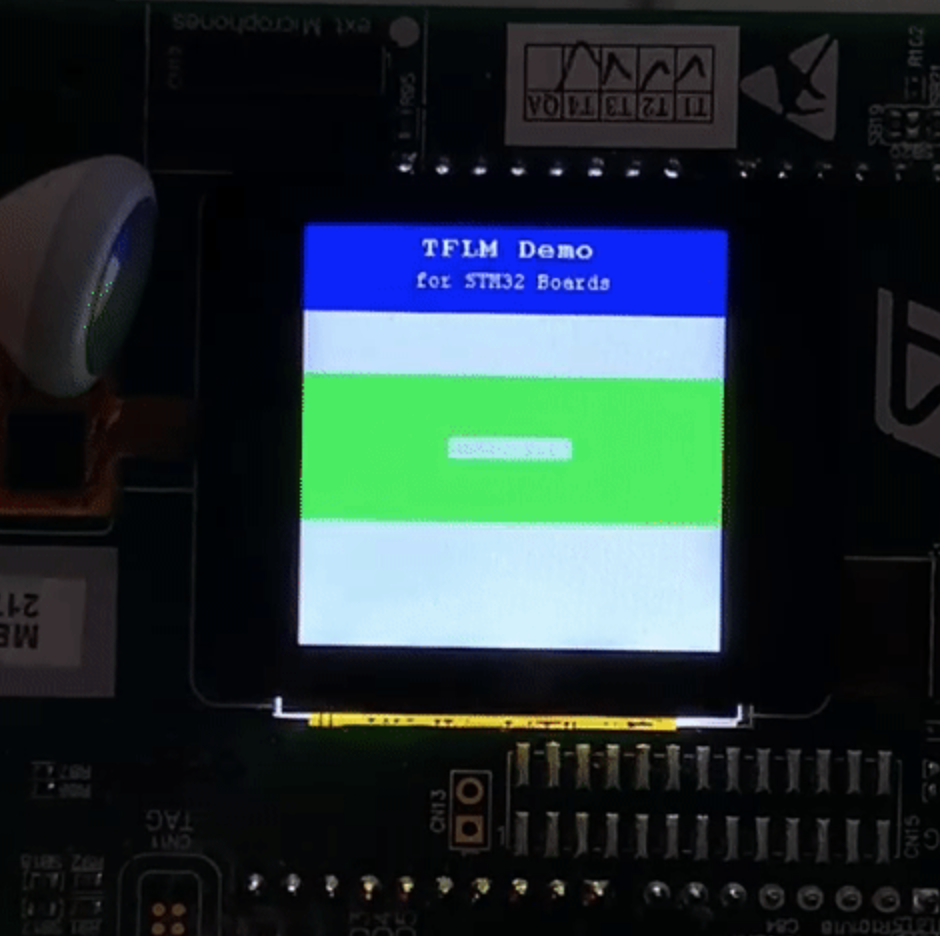
\includegraphics[width=0.8\textwidth]{figures/micro_speech_gif.png}
%         \caption{Micro Speech}
%         \label{fig:gif_mirco_speech}
%     \end{subfigure}
%     \hfill
%     \begin{subfigure}[b]{0.3\textwidth}
%         \centering
%         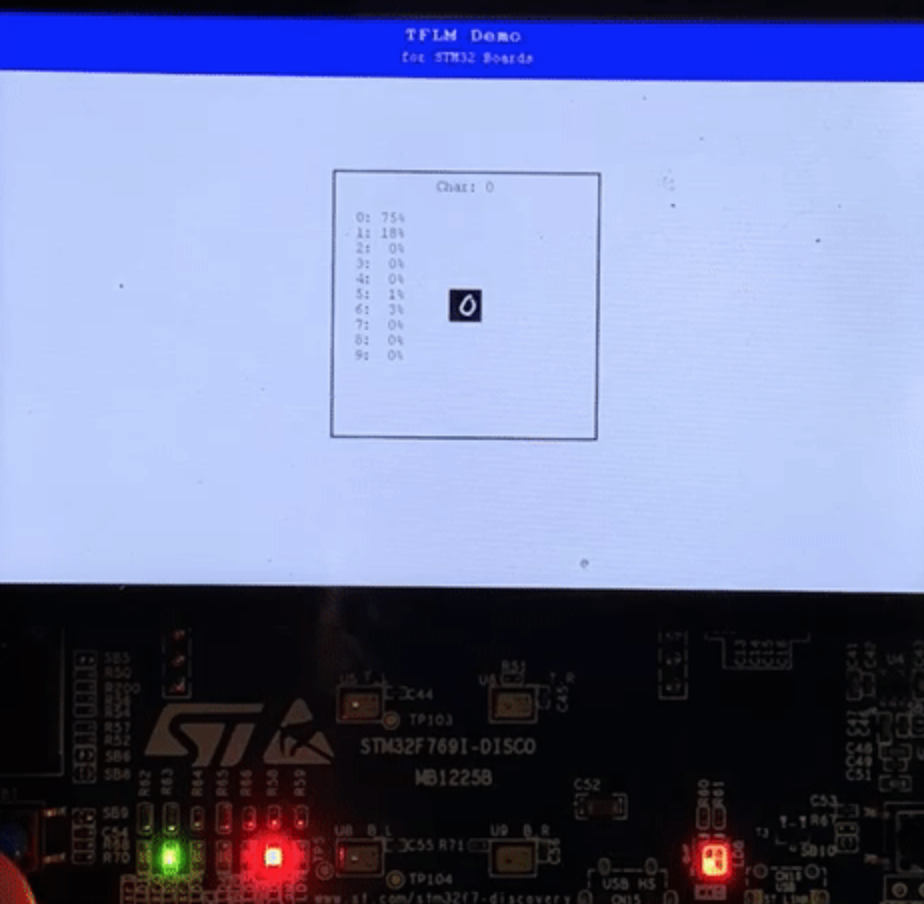
\includegraphics[width=0.8\textwidth]{figures/mnist_gif.png}
%         \caption{MNIST}
%         \label{fig:gif_mnist}
%     \end{subfigure}
%        \caption{Examples running on the STM32 Boards}
%        \label{fig:gifs}
%\end{figure}

\end{frame}

\begin{frame}
  \frametitle{Documentation}
  
  \centering{
  \begin{itemize}
      \item Common toolchain parts as submodules $\Rightarrow$ less redundant code
      \item Wrapper repository\footnote{\url{https://github.com/PhilippvK/stm32-tflm-demos}}
      \item Common documentation at a single place
      \item Great Extend-ability
  \end{itemize}}
  
  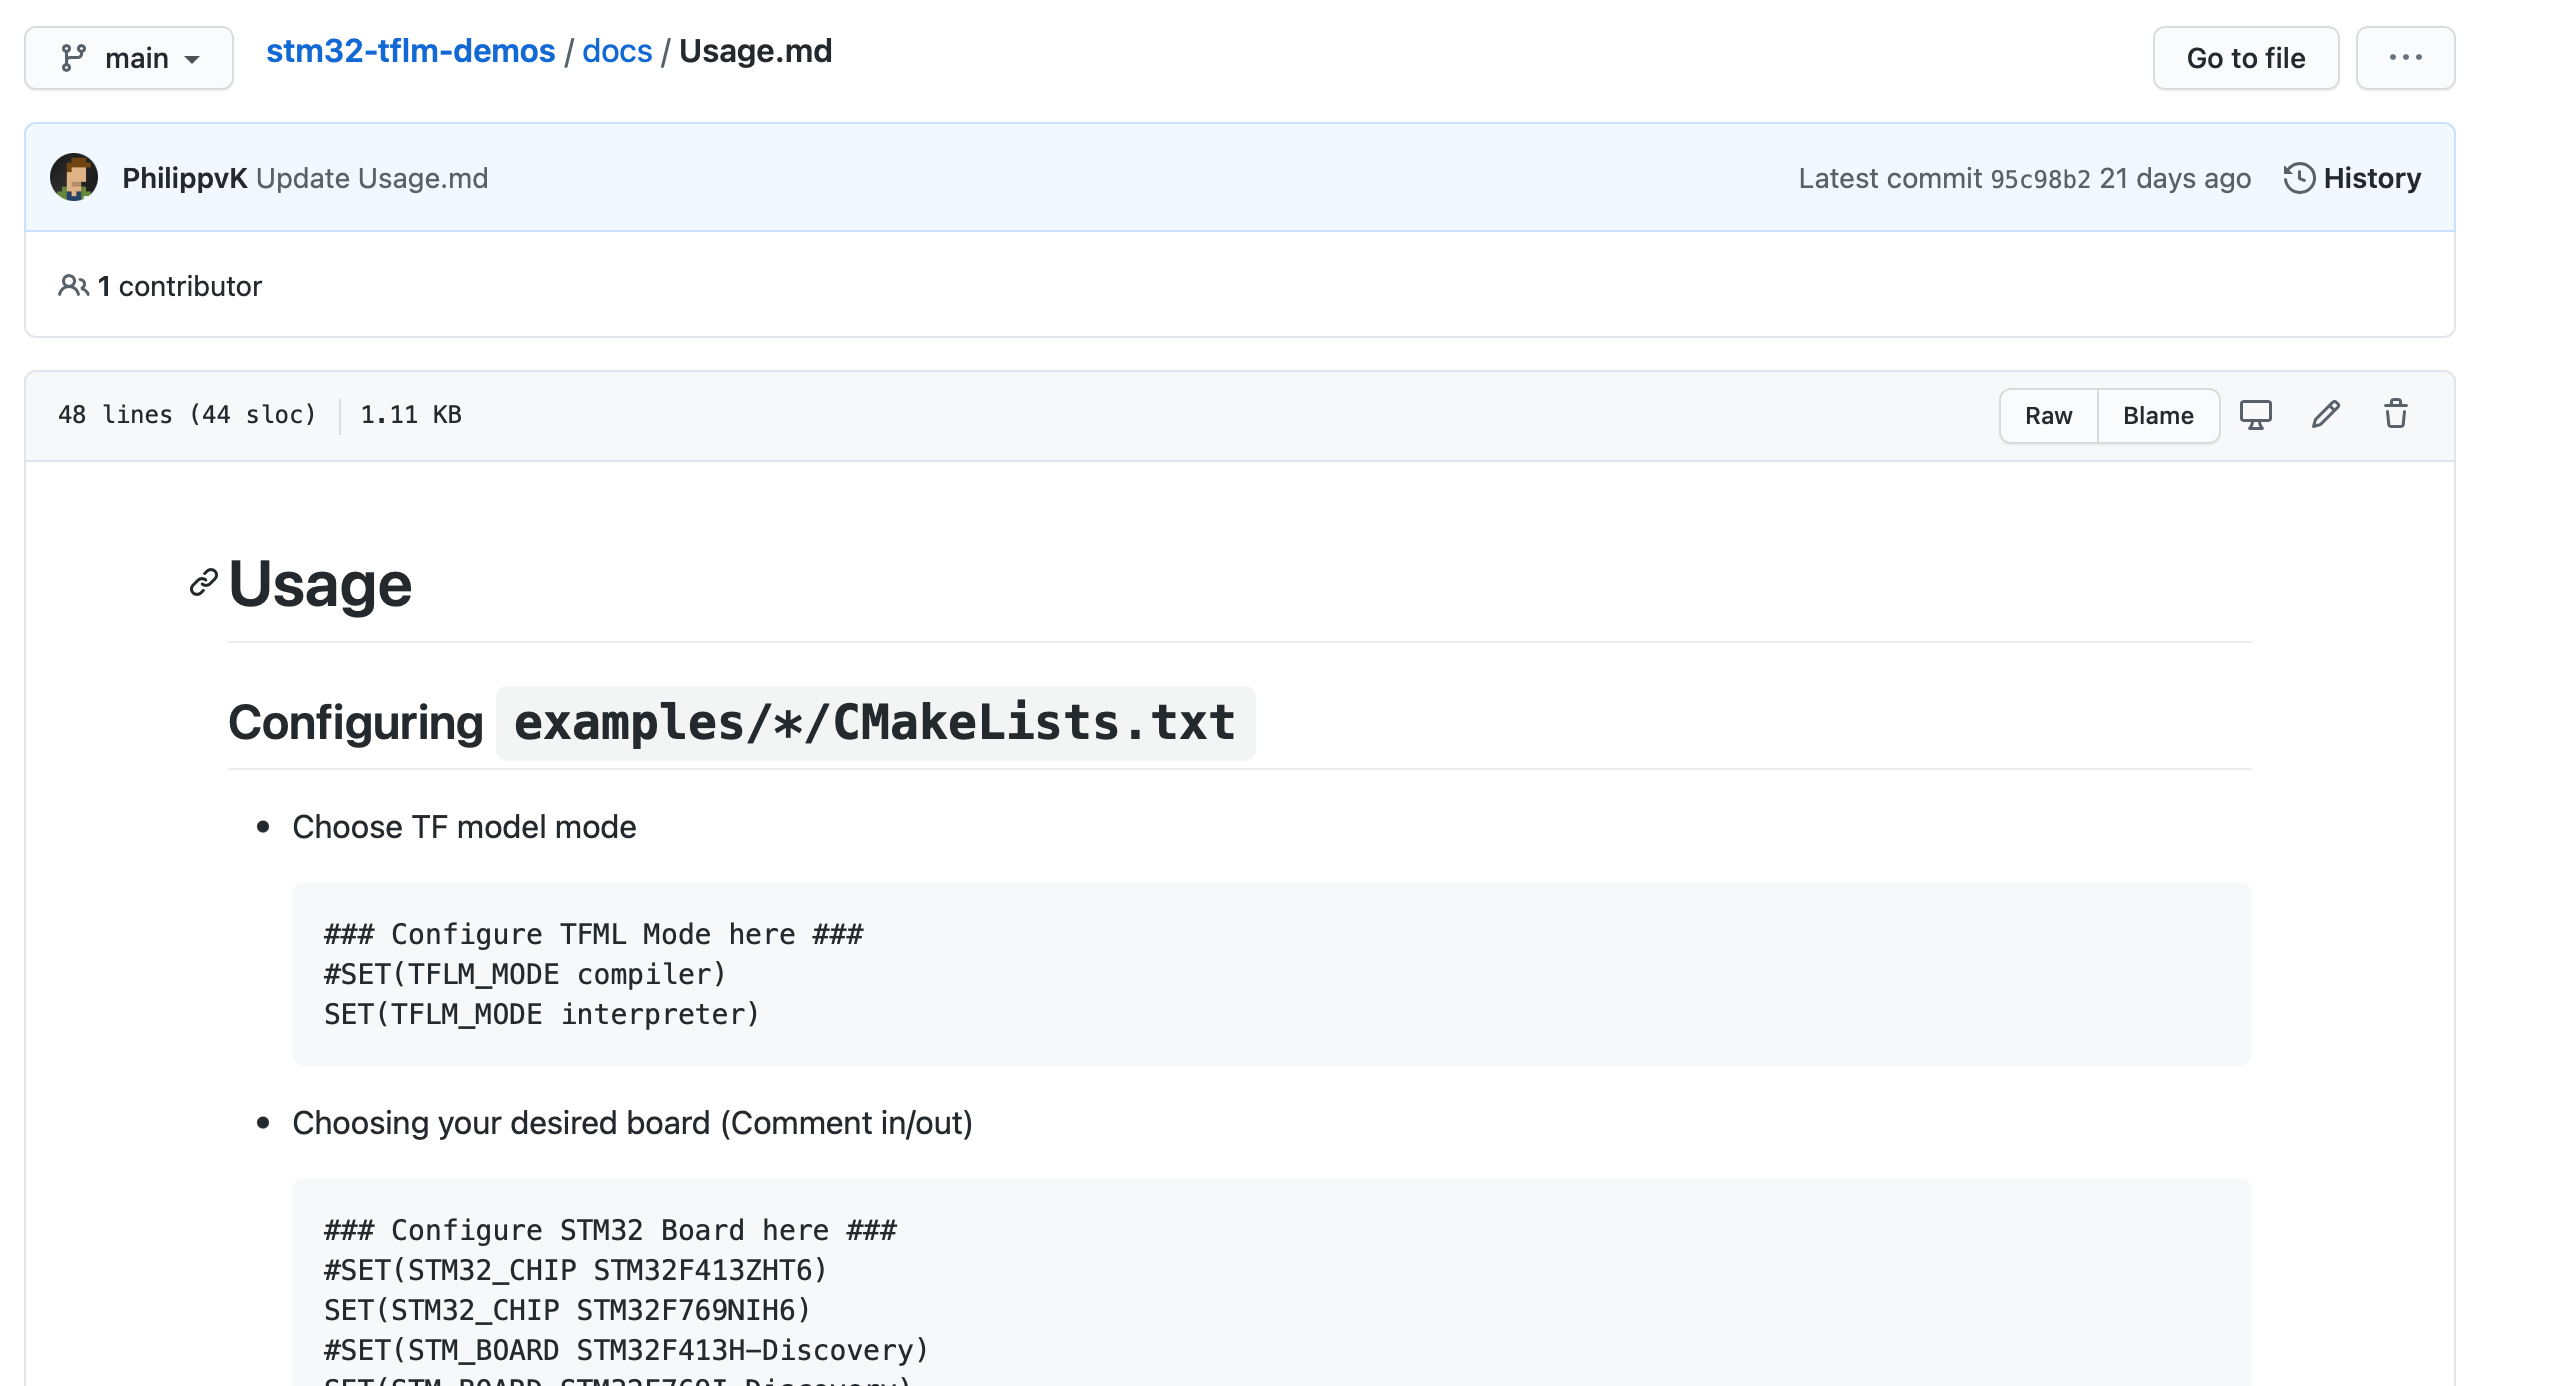
\includegraphics[width=.5\textwidth]{figures/docs.png}

\end{frame}

\begin{frame}
  \frametitle{Evaluation}
  % TODO: Board Metrics
  %\footfullcite{jirauschek2014}

\end{frame}

\begin{frame}
  \frametitle{Evaluation - Memory Usage}

  %\footfullcite{jirauschek2014}

\end{frame}

\begin{frame}
  \frametitle{Evaluation - Number of Ops}

  %\footfullcite{jirauschek2014}

\end{frame}

\begin{frame}
  \frametitle{Evaluation - Runtime Measurements}

  %\footfullcite{jirauschek2014}

\end{frame}

\begin{frame}
  \frametitle{Evaluation - CMSIS-NN Optimizations}

  %\footfullcite{jirauschek2014}

\end{frame}

\begin{frame}
  \frametitle{Conclusions and Outlook}

  \begin{itemize}
  \item Conclusion 1
  \item Conclusion 2
  \end{itemize}

  \pause

  \begin{itemize}
  \item Outlook 1
  \item Outlook 2
  \end{itemize}

\end{frame}

\begin{frame}
  \frametitle{Acknowledgments}

  We would like to thank...

  \begin{itemize}
  \item ... our students.
  \item ... the German Research Foundation (DFG) for funding.
    \vspace{2cm}
  \item \textbf{... you for your attention!}
  \end{itemize}
\end{frame}

\begin{frame}
  \frametitle{References}

  \printbibliography

\end{frame}

\end{document}
